%%%%%%%%%%%%%%%%%%%%%%%%%%%%%%%%%%%%%
%                                   %
% Compile with XeLaTeX and biber    %
%                                   %
% Questions or comments:            %
%                                   %
% joshua dot mcneill at uga dot edu %
%                                   %
%%%%%%%%%%%%%%%%%%%%%%%%%%%%%%%%%%%%%

\documentclass{beamer}
  % Read in standard preamble (cosmetic stuff)
  %%%%%%%%%%%%%%%%%%%%%%%%%%%%%%%%%%%%%%%%%%%%%%%%%%%%%%%%%%%%%%%%
% This is a standard preamble used in for all slide documents. %
% It basically contains cosmetic settings.                     %
%                                                              %
% Joshua McNeill                                               %
% joshua dot mcneill at uga dot edu                            %
%%%%%%%%%%%%%%%%%%%%%%%%%%%%%%%%%%%%%%%%%%%%%%%%%%%%%%%%%%%%%%%%

% Beamer settings
% \usetheme{Berkeley}
\usetheme{CambridgeUS}
% \usecolortheme{dove}
% \usecolortheme{rose}
\usecolortheme{seagull}
\usefonttheme{professionalfonts}
\usefonttheme{serif}
\setbeamertemplate{bibliography item}{}

% Packages and settings
\usepackage{fontspec}
  \setmainfont{Charis SIL}
\usepackage{hyperref}
  \hypersetup{colorlinks=true,
              allcolors=blue}
\usepackage{graphicx}
  \graphicspath{{../../figures/}}
\usepackage[normalem]{ulem}
\usepackage{enumerate}

% Document information
\author{M. McNeill}
\title[FREN2001]{Français 2001}
\institute{\url{joshua.mcneill@uga.edu}}
\date{}

%% Custom commands
% Lexical items
\newcommand{\lexi}[1]{\textit{#1}}
% Gloss
\newcommand{\gloss}[1]{`#1'}
\newcommand{\tinygloss}[1]{{\tiny`#1'}}
% Orthographic representations
\newcommand{\orth}[1]{$\langle$#1$\rangle$}
% Utterances (pragmatics)
\newcommand{\uttr}[1]{`#1'}
% Sentences (pragmatics)
\newcommand{\sent}[1]{\textit{#1}}
% Base dir for definitions
\newcommand{\defs}{../definitions}


  % Packages and settings

  % Document information
  \subtitle[Indéfinies et négatives]{Les expressions indéfinies et négatives}

\begin{document}
  % Read in the standard intro slides (title page and table of contents)
  \begin{frame}
    \titlepage
    \tiny{Office: % Basically a variable for office hours location
Gilbert 121\\
          Office hours: % Basically a variable for office hours
 lundi, mercredi, vendredi 10:10--11:10
}
  \end{frame}

  \begin{frame}{Les verbes comme \lexi{voir}}
    \begin{center}
      \begin{tabular}{l | l l | l l}
  \multicolumn{5}{c}{voir \gloss{to see}} \\
  \hline
      & \multicolumn{2}{l |}{singulier} & \multicolumn{2}{l}{pluriel} \\
  \hline
  1re & je         & vois               & nous        & vo\alert{y}ons \\
  2e  & tu         & vois               & vous        & vo\alert{y}ez \\
  \hline
  3e  & il (masc)  &                    & ils (masc)  & \\
      & elle (fem) & voit               & elles (fem) & voient \\
      & on         &                    &             & \\
  \hline
  \multicolumn{5}{c}{Impératifs $\to$ vois, voyez, voyons} \\
  \multicolumn{5}{c}{Passé composé $\to$ j'ai vu} \\
  \multicolumn{5}{c}{Futur simple $\to$ je v\alert{err}ai}
\end{tabular}

    \end{center}
    \lexi{Croire} au futur simple $\to$ \lexi{je croirai}
  \end{frame}

  \begin{frame}{Quelque chose ou rien}
    \begin{columns}
      \column{0.5\textwidth}
        \begin{enumerate}
          \item On a vu \alert{quelque chose} sur la table?
          \item<2->[$\to$] Non, on n'a \alert{rien} vu sur la table.
          \item<3-> \alert{Quelqu'un} lui téléphone?
          \item<4->[$\to$] Non, \alert{personne ne} lui téléphone.
          \item<5-> Il y a \alert{quelqu'un} à la porte?
          \item<6->[$\to$] Oui, il y a \alert{quelqu'un} à la porte.
          \item<7-> Tu vas manger au Grit \alert{quelquefois}?
          \item<8->[$\to$] Non, je ne vais \alert{jamais} manger au Grit.
          \item<9-> Il va donner \textcolor{red}{quelque chose} à \textcolor{purple}{quelqu'un}?
          \item<10->[$\to$] Non, il ne va \textcolor{red}{rien} donner à \textcolor{purple}{personne}.
        \end{enumerate}
      \column{0.5\textwidth}
        \begin{minipage}[c][0.8\textheight]{\linewidth}
          \begin{center}
            \only<1-2>{
              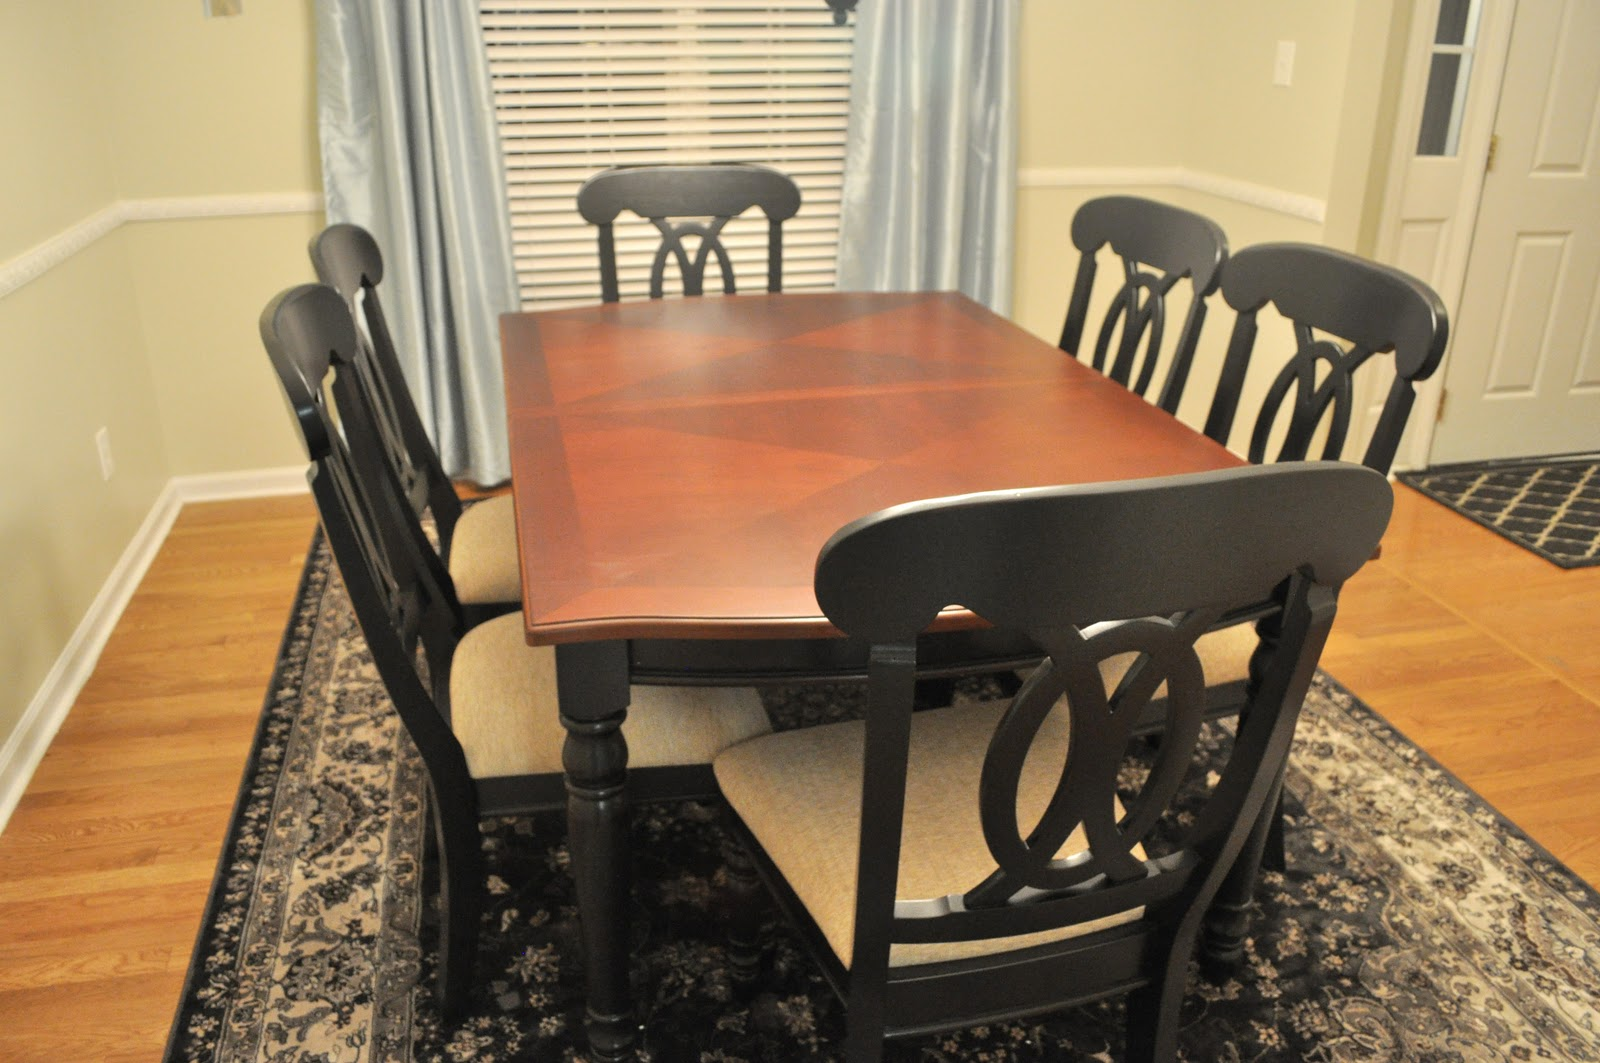
\includegraphics[scale=0.5]{table.jpg}
            }
            \only<3-4>{
              
\includegraphics[scale=0.5]{téléphone.jpg}
            }
            \only<5-6>{
              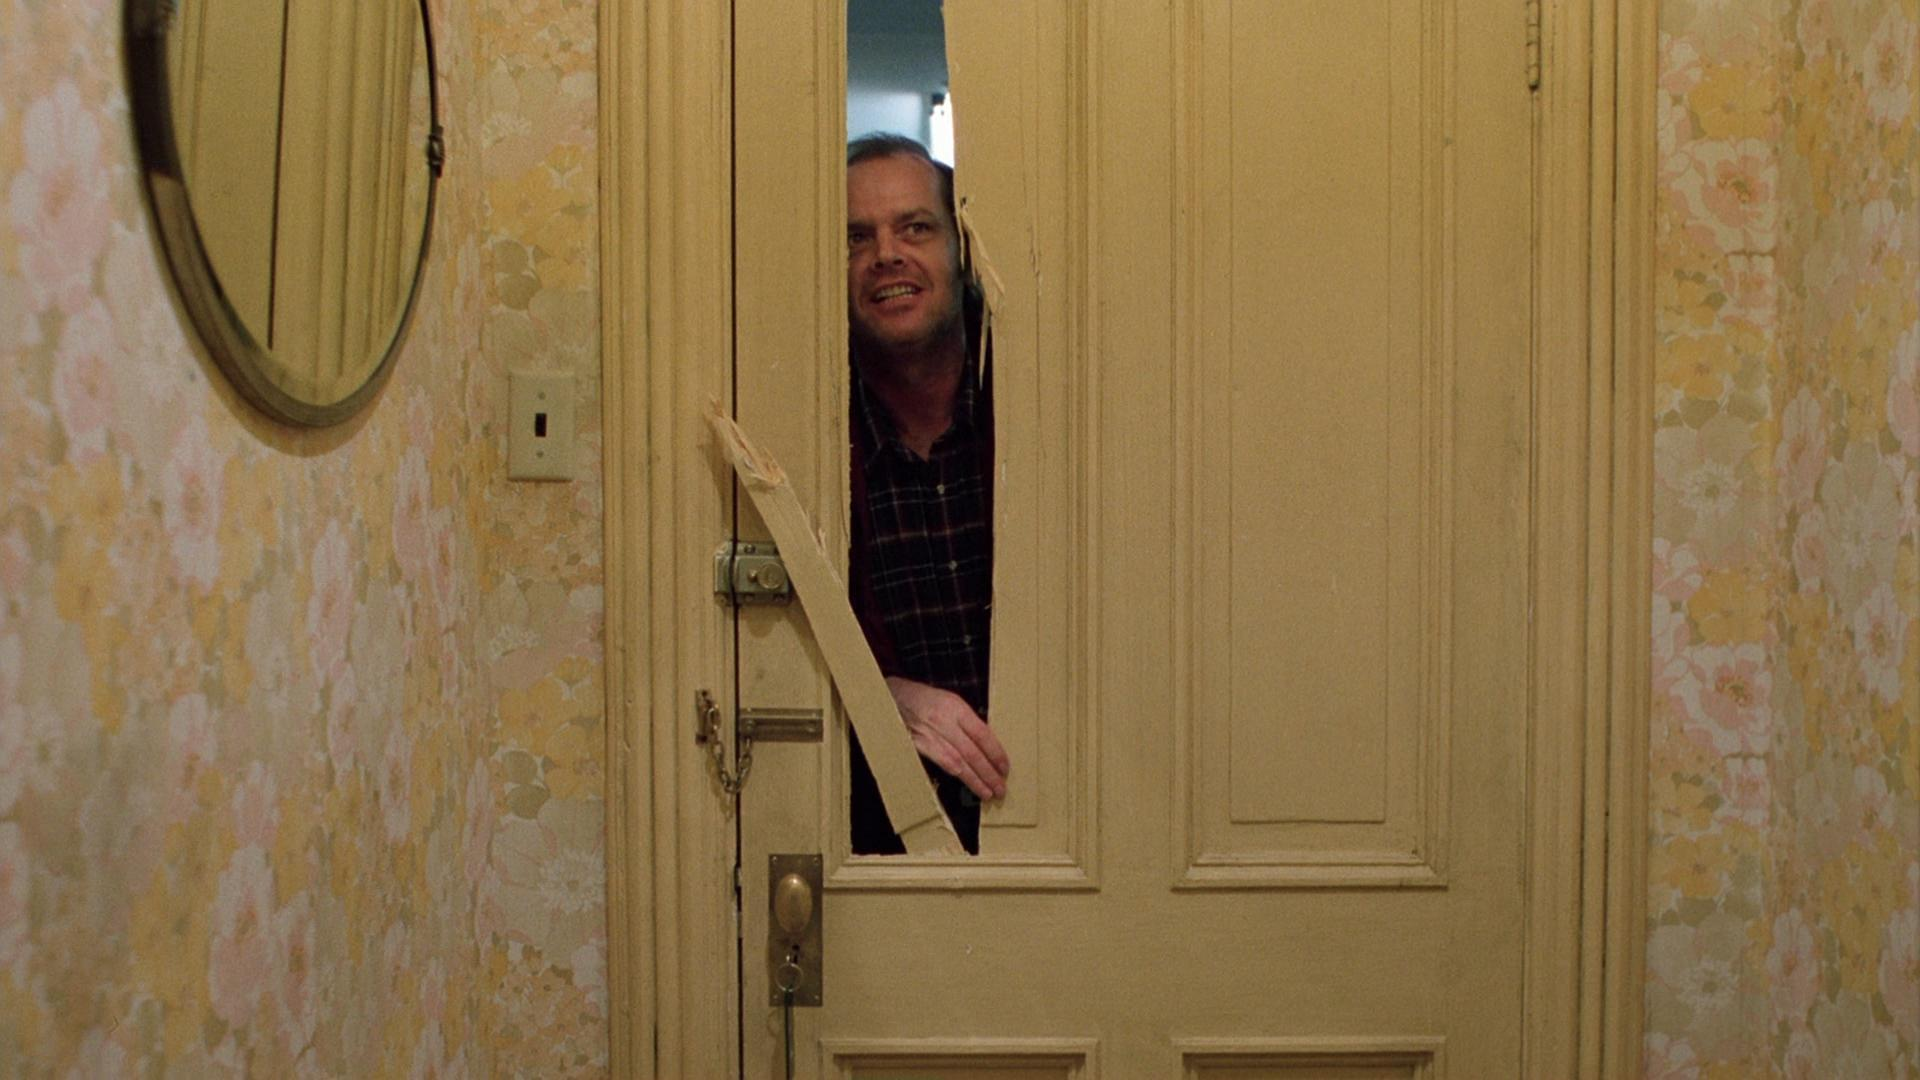
\includegraphics[scale=0.5]{porte.jpg}
            }
            \only<7-8>{
              
\includegraphics[scale=0.5]{grit.jpg}
            }
            \only<9-10>{
              
\includegraphics[scale=0.5]{bezos.jpg}
            }
          \end{center}
        \end{minipage}
    \end{columns}
  \end{frame}

  \begin{frame}{}
    \begin{center}
      \Large Quiz
    \end{center}
  \end{frame}

  \begin{frame}{Quand ça arrive}
    Avec un/e partenaire, échangez vos réponses aux questions suivantes.
    Utilisez les expressions indéfinies (\lexi{quelquefois}, \lexi{quelque chose}, \lexi{quelqu'un}) et négatives (\lexi{ne...jamais}, \lexi{ne...rien}, \lexi{ne...personne}).
    \begin{description}
      \item[] \textbf{Modèle:} \emph{Quand vous allez au supermarché}
      \item[E1:] \emph{Je crois que} la politesse est plus importante. Si on est poli, ...
      \item[E2:] Moi, \emph{je ne crois pas}. Il faut être honnête parce que ...
    \end{description}
    \begin{columns}[t]
      \column{0.5\textwidth}
        \begin{enumerate}
          \item la politesse ou l'honnêteté
          \item l'individualisme ou la solidarité
          \item la tradition ou l'indépendance
        \end{enumerate}
      \column{0.5\textwidth}
        \begin{enumerate}
          \setcounter{enumi}{3}
          \item le bien commun ou le succès personnel
          \item la créativité ou la discipline
          \item la recherche spirituelle ou les pratiques religieuses
        \end{enumerate}
    \end{columns}
  \end{frame}

  \begin{frame}{}
    \begin{center}
      \Large Questions?
    \end{center}
  \end{frame}
\end{document}
